
\documentclass[compress]{beamer}
\usepackage{ifthen,verbatim}

\newcommand{\isnote}{}
\xdefinecolor{lightyellow}{rgb}{1.,1.,0.25}
\xdefinecolor{darkblue}{rgb}{0.1,0.1,0.7}
\xdefinecolor{gray}{rgb}{0.5,0.5,0.5}

%% Uncomment this to get annotations
%% \def\notes{\addtocounter{page}{-1}
%%            \renewcommand{\isnote}{*}
%% 	   \beamertemplateshadingbackground{lightyellow}{white}
%%            \begin{frame}
%%            \frametitle{Notes for the previous page (page \insertpagenumber)}
%%            \itemize}
%% \def\endnotes{\enditemize
%% 	      \end{frame}
%%               \beamertemplateshadingbackground{white}{white}
%%               \renewcommand{\isnote}{}}

%% Uncomment this to not get annotations
\def\notes{\comment}
\def\endnotes{\endcomment}

\setbeamertemplate{navigation symbols}{}
\setbeamertemplate{headline}{\mbox{ } \hfill
\begin{minipage}{5.5 cm}
\vspace{-0.75 cm} \small
\end{minipage} \hfill
\begin{minipage}{4.5 cm}
\vspace{-0.75 cm} \small
\begin{flushright}
\ifthenelse{\equal{\insertpagenumber}{1}}{}{Jim Pivarski \hspace{0.2 cm} \insertpagenumber\isnote/\pageref{numpages}}
\end{flushright}
\end{minipage}\mbox{\hspace{0.2 cm}}\includegraphics[height=1 cm]{../cmslogo} \hspace{0.1 cm} \includegraphics[height=1 cm]{../tamulogo} \hspace{0.01 cm} \vspace{-1.05 cm}}

\begin{document}
\begin{frame}
\vfill
\begin{center}
\textcolor{darkblue}{\Large Proposal for Muon Alignment AlCaRecos}

\vfill
\begin{columns}
\column{0.3\linewidth}
\begin{center}
\large
\textcolor{darkblue}{Jim Pivarski}
\end{center}
\end{columns}

\begin{columns}
\column{0.3\linewidth}
\begin{center}
\scriptsize
{\it Texas A\&M University}
\end{center}
\end{columns}

\vfill
28 October, 2008

\end{center}
\end{frame}

%% \begin{notes}
%% \item This is the annotated version of my talk.
%% \item If you want the version that I am presenting, download the one
%% labeled ``slides'' on Indico (or just ignore these yellow pages).
%% \item The annotated version is provided for extra detail and a written
%% record of comments that I intend to make orally.
%% \item Yellow notes refer to the content on the {\it previous} page.
%% \item All other slides are identical for the two versions.
%% \end{notes}

\small

\begin{frame}
\frametitle{AlCaRecos for collisions MC}
\scriptsize
\renewcommand{\arraystretch}{1.2}

\begin{tabular}{p{0.3\linewidth} p{0.2\linewidth} p{0.4\linewidth}}
Muon AlCaReco Stream & Dataset & Comments \\\hline
MuAlCalIsolatedMu & Express Stream

step 2 & Main muon source for two alignment algorithms, DT calibration \\
MuAlOverlaps & Express Stream

step 3 or Prompt Reco & Optimized for CSC overlaps algorithm (reduction $\sim$factor 50) \\
\textcolor{gray}{MuAlZMuMu} & \textcolor{gray}{Prompt Reco or}

\textcolor{gray}{not at all} & \textcolor{gray}{Monthly timescale, at least at first; no algorithm currently defined to use mass constraint} \\
\end{tabular}

\vfill
\hspace{-0.83 cm} \textcolor{darkblue}{\Large AlCaRecos for data and special MC samples}

\begin{tabular}{p{0.3\linewidth} p{0.2\linewidth} p{0.4\linewidth}}
Muon AlCaReco Stream & Dataset & Comments \\\hline
\textcolor{darkblue}{Same as above, plus\ldots} & & \\
MuAlStandAloneCosmics & Prompt Reco & Important for alignment, but requires special reconstruction \\
MuAlGlobalCosmics & Prompt Reco & These are tracker-pointing globalMuons \\
MuAlBeamHalo & Prompt Reco & Triggered by CSC beam-halo trigger instead of RPC cosmics \\
MuAlBeamHaloOverlaps & Prompt Reco & Same overlaps selection applied to non-collisions \\
\end{tabular}

\vfill
If Cosmics and BeamHalo primary datasets are combined, then \mbox{MuAlStandAloneCosmics\hspace{-0.5 cm}} and MuAlBeamHalo could be combined.  They are not distinguished by purpose.

%% \hspace{-0.83 cm} \textcolor{darkblue}{\Large Outline2}
\label{numpages}
\end{frame}

%% \begin{frame}
%% \frametitle{Some context}

%% \begin{itemize}
%% \item Only Prompt Reco can have non-standard reconstruction paths

%% \mbox{ } \hfill 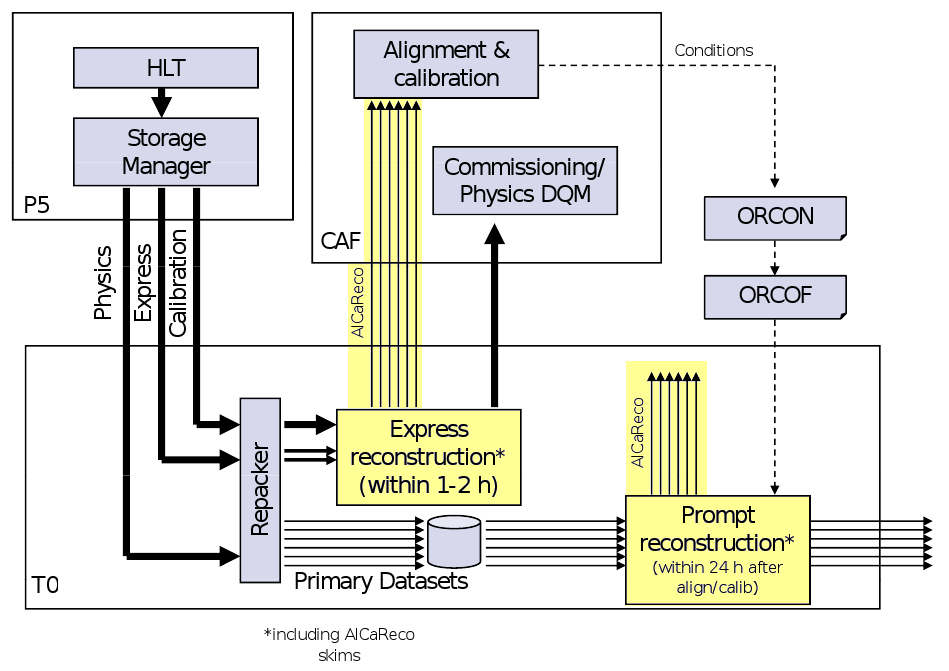
\includegraphics[width=0.6\linewidth]{alcareco_path.png} \hfill \mbox{ }

%% \item HLT selection is not a question of algorithmic speed, \mbox{but backgrounds\hspace{-1 cm}}

%% \mbox{ } \hfill 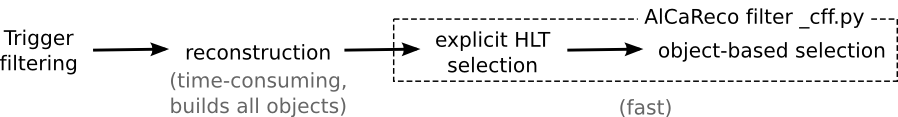
\includegraphics[width=0.8\linewidth]{alca_path2.png} \hfill \mbox{ }

%% \item Do HLT filters reject more backgrounds than the AlCa
%%   object-based selection?  Could that processing be replicated in the
%%   AlCa step?

%% \end{itemize}
%% \end{frame}

%% \section*{First section}
%% \begin{frame}
%% \begin{center}
%% \Huge \textcolor{blue}{First section}
%% \end{center}
%% \end{frame}

%% \begin{frame}
%% \label{numpages}
%% \end{frame}

\end{document}
